%%%%%%%%%%%%%%%%%%%%%%%%%%%%%%%%%%%%%%%%%
% Journal Article
% LaTeX Template
% Version 1.4 (15/5/16)
%
% This template has been downloaded from:
% http://www.LaTeXTemplates.com
%
% Original author:
% Frits Wenneker (http://www.howtotex.com) with extensive modifications by
% Vel (vel@LaTeXTemplates.com)
%
% License:
% CC BY-NC-SA 3.0 (http://creativecommons.org/licenses/by-nc-sa/3.0/)
%
%%%%%%%%%%%%%%%%%%%%%%%%%%%%%%%%%%%%%%%%%

%----------------------------------------------------------------------------------------
%	PACKAGES AND OTHER DOCUMENT CONFIGURATIONS
%----------------------------------------------------------------------------------------

\documentclass[10pt]{article} % Single column

%\documentclass[twoside,twocolumn]{article} % Two column

\usepackage{blindtext} % Package to generate dummy text throughout this template 

\usepackage[sc]{mathpazo} % Use the Palatino font
\usepackage[T1]{fontenc} % Use 8-bit encoding that has 256 glyphs
\linespread{1.05} % Line spacing - Palatino needs more space between lines
\usepackage{microtype} % Slightly tweak font spacing for aesthetics

\usepackage[spanish]{babel} % Language hyphenation and typographical rules

\usepackage[hmarginratio=1:1,top=32mm,columnsep=20pt]{geometry} % Document margins
\usepackage[hang, small,labelfont=bf,up,textfont=it,up]{caption} % Custom captions under/above floats in tables or figures
\usepackage{booktabs} % Horizontal rules in tables

\usepackage{lettrine} % The lettrine is the first enlarged letter at the beginning of the text

\usepackage{enumitem} % Customized lists
\setlist[itemize]{noitemsep} % Make itemize lists more compact

\usepackage{abstract} % Allows abstract customization
\renewcommand{\abstractnamefont}{\normalfont\bfseries} % Set the "Abstract" text to bold
\renewcommand{\abstracttextfont}{\normalfont\small\itshape} % Set the abstract itself to small italic text

\usepackage{titlesec} % Allows customization of titles
\renewcommand\thesection{\Roman{section}} % Roman numerals for the sections
\renewcommand\thesubsection{\roman{subsection}} % roman numerals for subsections
\titleformat{\section}[block]{\large\scshape\centering}{\thesection.}{1em}{} % Change the look of the section titles
\titleformat{\subsection}[block]{\large}{\thesubsection.}{1em}{} % Change the look of the section titles

\usepackage{fancyhdr} % Headers and footers
\pagestyle{fancy} % All pages have headers and footers
\fancyhead{} % Blank out the default header
\fancyfoot{} % Blank out the default footer
\fancyhead[C]{Sistemas Distribuidos. \textbf{Monica Scheduler}} % Custom header text
\fancyfoot[RO,LE]{\thepage} % Custom footer text

\usepackage{titling} % Customizing the title section

\usepackage{hyperref} % For hyperlinks in the PDF

\usepackage{graphicx} % For images

\usepackage{pifont} % bullets

\usepackage{amsmath}

\usepackage{algpseudocode}

\usepackage{float}
% Keywords command
\providecommand{\keywords}[1]
{
	\small	
	\vspace{0.5em}
	\noindent \textbf{\textit{Palabras clave --- }} #1
}


%----------------------------------------------------------------------------------------
%	TITLE SECTION
%----------------------------------------------------------------------------------------

\setlength{\droptitle}{-4\baselineskip} % Move the title up

\pretitle{\begin{center}\Huge\bfseries} % Article title formatting
	\posttitle{\end{center}} % Article title closing formatting
\title{\normalsize{Sistemas Distribuidos}\\
	\Huge\bfseries Monica Scheduler \\
} % Article title
\author{% 
	% \includegraphics[width=15em]{logo.png}\\
	Laura Victoria Riera P\'erez\\
	Mari\'e del Valle Reyes \vspace{1em} \\
	\small Cuarto a\~no. Ciencias de la Computaci\'on. \\ % institution
	\small Facultad de Matem\'atica y Computaci\'on, Universidad de La Habana, Cuba \\ % institution
}
\date{\footnotesize \today } % Leave empty to omit a date


% Abstract configurations
\renewenvironment{abstract}
{\small
	\begin{center}
		\bfseries \abstractname\vspace{-.5em}\vspace{0pt}
	\end{center}
	\list{}{
		\setlength{\leftmargin}{1.5cm}%
		\setlength{\rightmargin}{\leftmargin}%
	}%
	\item\relax}
{\endlist}

\usepackage{amsthm}
\usepackage{amssymb}
\usepackage{todonotes} % \TODO
\usepackage{listings} % Code listings
\usepackage{xcolor}

\definecolor{backcolour}{rgb}{0.95,0.95,0.92}

\newcommand{\csl}[1]{\colorbox{backcolour}{\texttt{#1}}}

\newcommand{\imgcaption}[2]{\tiny \textbf{Figura #1.} #2.}

\newcommand{\mgc}[2][]{\colorbox{backcolour}{\texttt{\_\_#2\_\_#1}}}

\newcommand{\mgccapt}[1]{\texttt{\_\_#1\_\_}}

\newtheorem{thm}{Teorema}
\newtheorem{mydef}{Definici\'on}%[section]
\newtheorem{lem}{Lema}
\newtheorem{fig}{\scriptsize{Figura}}


\renewcommand{\qedsymbol}{\rule{0.7em}{0.7em}}

% Hyperlinks configurations
\hypersetup{
	colorlinks=true,
	linkcolor=black,
	filecolor=magenta,      
	urlcolor=cyan,
	pdftitle={Overleaf Example},
	pdfpagemode=FullScreen,
}

%----------------------------------------------------------------------------------------

\begin{document}
	
	\bibliographystyle{ieeetr}
	
	% Print the title
	\maketitle
	
	%----------------------------------------------------------------------------------------
	%	ARTICLE CONTENTS
	%----------------------------------------------------------------------------------------
	
	\section*{Repositorio del proyecto}
	
	\begin{center}
		\href{https://github.com/computer-science-crows/monica-scheduler}{https://github.com/computer-science-crows/monica-scheduler}
	\end{center}

	Implementación de una Agenda Electrónica como Sistema Distribuido con DHT Kademlia
	
	\section{Introducción}
	
	El tiempo es un recurso invaluable y su gestión eficiente es esencial para la productividad y el bienestar personal. Una estrategia comúnmente utilizada para la gestión del tiempo es el uso de una agenda. Sin embargo, en muchas ocasiones, es necesario coordinar dicha agenda con otras personas para llevar a cabo actividades conjuntas. Este proceso implica la identificación de horarios compartidos y la detección de intervalos de tiempo libres. Además, estas planificaciones pueden verse alteradas por eventos imprevistos que requieren asistencia, lo que conlleva la necesidad de modificar la agenda nuevamente.
	
	Para abordar estos desafíos, este proyecto propone la creación de una agenda electrónica distribuida como herramienta de gestión del tiempo para eventos personales o grupales. El sistema se diseñó e implementó como un sistema distribuido, utilizado la Tabla Hash Distribuida (DHT) de Kademlia para la gestión de datos.
	
	\section{Requerimientos}
	
	Este proyecto consiste en crear una agenda distribuida como herramienta de gestión del tiempo para eventos personales o grupales. Los requisitos clave para este sistema son:
	
	\begin{itemize}
		\item \textbf{Arquitectura Distribuida}: El sistema debe ser diseñado e implementado como un sistema distribuido. Esto significa que el sistema debe ser capaz de funcionar en múltiples máquinas mientras se presenta a los usuarios como un sistema coherente único.
		
		\item \textbf{Mecanismo de Autenticación e Identificación}: El sistema debe ser capaz de autenticar e identificar a cada usuario. Esto asegura que solo los usuarios autorizados puedan acceder al sistema y realizar ciertas acciones.
		
		\item \textbf{Formación de Grupos}: El sistema debe permitir la creación de grupos, ya sean jerárquicos o no jerárquicos. Esto significa que los usuarios deben poder crear y gestionar grupos dentro del sistema de manera flexible.
		
		\item \textbf{Citas Grupales}: El sistema debe admitir la creación de citas grupales. Si se utiliza un grupo jerárquico, una cita creada por un superior debe aparecer automáticamente en las agendas de todos los miembros del grupo. Para grupos no jerárquicos, todos los miembros deben aceptar la cita para que se confirme.
		
		\item \textbf{Actualizaciones Automáticas de la Agenda}: Cuando se crea, modifica o elimina una cita, los cambios deben reflejarse automáticamente en las agendas de los usuarios relevantes.
		
		\item \textbf{Identificación de Conflictos}: El sistema debe ser capaz de identificar conflictos en las agendas locales. Por ejemplo, si un usuario tiene programadas dos citas al mismo tiempo, el sistema debe señalar esto como un conflicto.
		
	\end{itemize}
	
	\section{Arquitectura del Sistema}
	
	El sistema se compone de cuatro partes fundamentales: CLI, capa de negocio, capa que conecta la l\'ogica con la red y la red con los datos.
	
	\begin{center}
		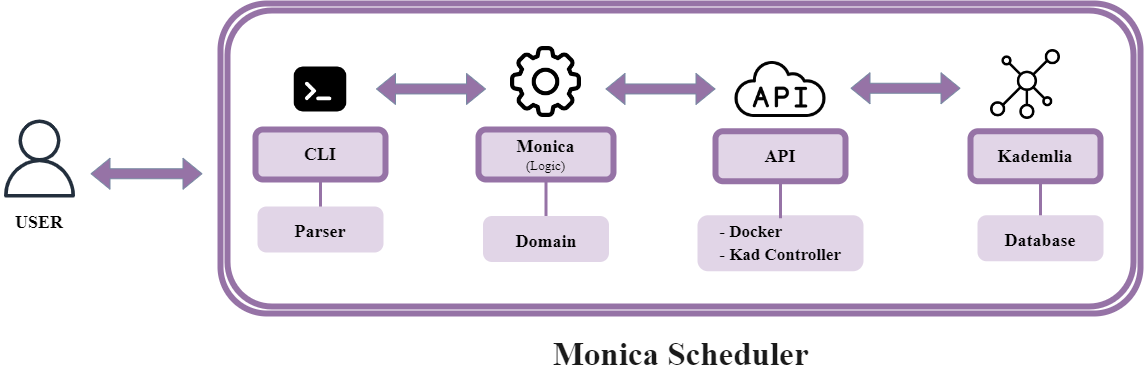
\includegraphics[scale=0.4]{esquema}
	\end{center}
	
	\subsection{CLI}
	
	Para la presentación y prueba del sistema, se desarrolló una interfaz de línea de comandos (CLI). Los usuarios pueden interactuar con el sistema a través de la CLI, lo que permite una interacción flexible y eficiente con el sistema. La lista de comandos y su descripci\'on se pueden observar al ejecutar el sistema e insertar el comando \texttt{-h} o \texttt{--help}.
	
	\subsection{L\'ogica de negocio}
	
	En la capa de negocio se implementaron las clases y m\'etodos necesarios para la representaci\'on de las entidades y relaciones que el problema se evidencian. Entre dichas entidades se encuantran:
	\begin{itemize}
		\item \textbf{User}: Representa a un usuario de la agenda distribuida.
		\item \textbf{Workspace}: Representa un grupo en la agenda distribuida. Los grupos pueden ser jer\'arquicos o no.
		\item \textbf{Event}: Representa un evento de un workspace en la agenda distribuida.
		\item \textbf{Request}: Representa una petici\'on o invitaci\'on que realizan los usuarios y se muestran como notificaciones. Se utilizan para invitar a usuarios a un grupo o aceptar la creaci\'on de un evento en grupos no jer\'arquicos.
	\end{itemize}

	\begin{center}
		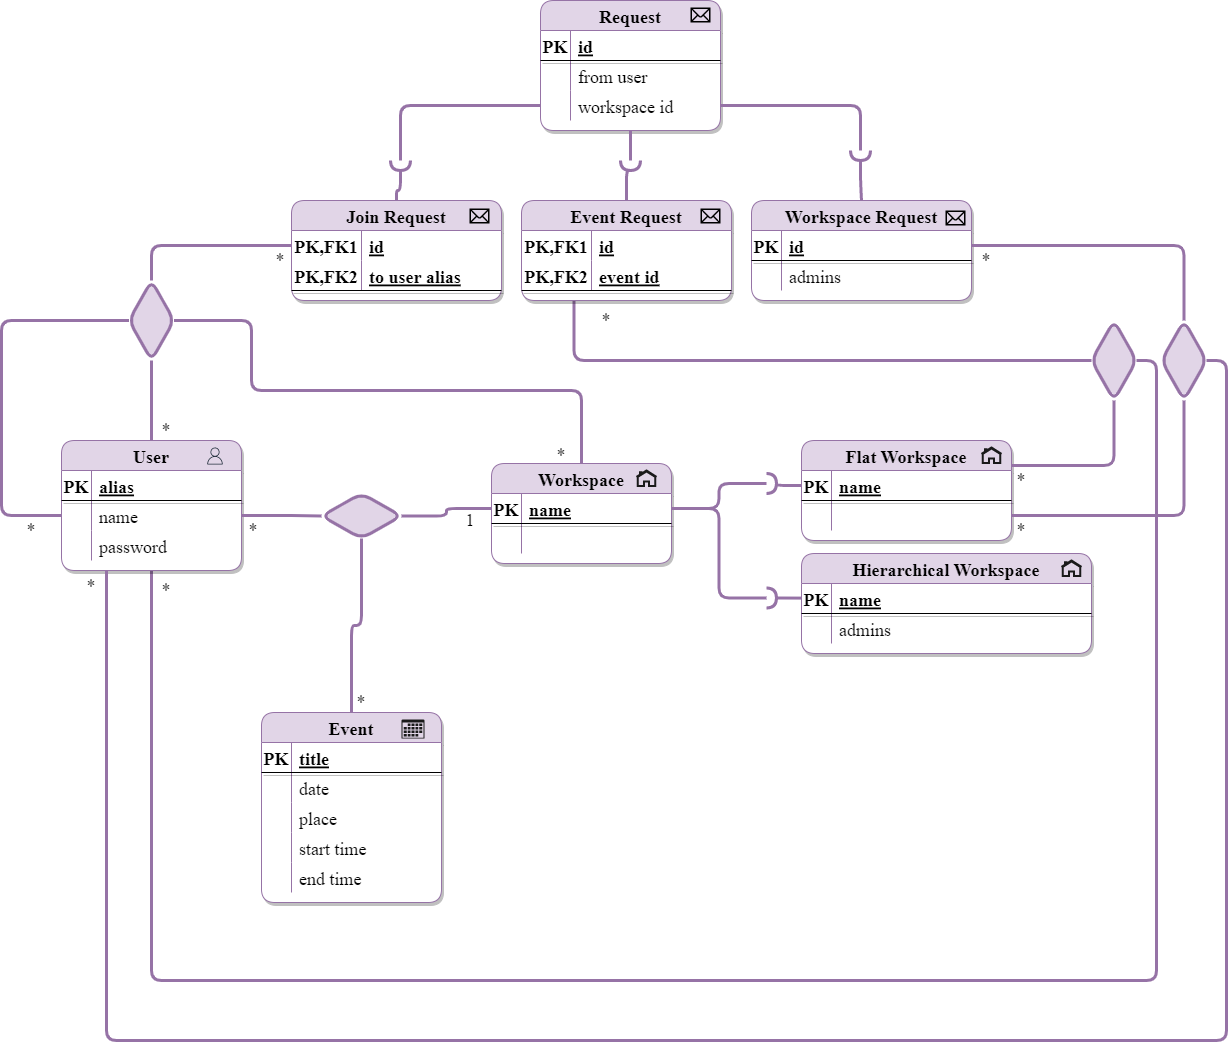
\includegraphics[scale=0.3]{modelo-merx}
	\end{center}
	

	
	\subsection{Capa intermedia}
	
	Esta capa se encarga de conectar la l\'ogica de negocio con la red de datos. Para ello se auxilia de m\'etodos \texttt{get()} y \texttt{set()} para pedir y guardar datos en la red.
	
	\subsection{Red de Kademlia}
	
	 Kademlia \cite{kad} es un protocolo de la capa de aplicación diseñado para redes P2P descentralizadas. En una de este tipo los nodos se distribuyen de forma descentralizada utilizando una estructura de árbol binario. 
	 
	El proceso de ingreso de un nodo a la red Kademlia se realiza mediante un mecanismo de broadcast. Cuando un nuevo nodo se quiere unir a la red, envía un mensaje de broadcast a todos los nodos existentes. Si hay algun servidor escuchando este devolvera su ip, lo cual permitira al nodo poder conectarse a la red. Los nodos existentes actualizan sus tablas de enrutamiento para incluir al nuevo nodo.
	 
	Para realizar búsquedas en la red, se utiliza un algoritmo basado en DHT (Distributed Hash Table). El algoritmo busca los k nodos más cercanos (en términos de distancia XOR) a una clave específica. Comienza seleccionando $\alpha$ contactos de los k cubetas que contienen nodos más cercanos a la clave buscada. Luego, envía mensajes asincrónicos a estos contactos para obtener información sobre la clave. Cada contacto activo devuelve información que ayuda a acercarse al nodo objetivo. Este proceso se repite hasta que se encuentra el nodo deseado.	
	 
	 Por otra parte, para el almacenamiento de los datos se utiliz\'o la librer\'ia \texttt{dictdatabase}, la cual proporciona m\'etodos para obtener y guardar datos en archivos \textit{.json}.
		
	En cuanto a la tolerancia a fallos, Kademlia utiliza una estructura descentralizada que proporciona una fuerte defensa contra ataques de denegación de servicio. Debido a la distribución de los nodos y la redundancia de la información en la red, es difícil para un atacante afectar el funcionamiento de toda la red. Además, Kademlia permite que los nodos se unan y abandonen la red de forma independiente, lo que proporciona flexibilidad y adaptabilidad a cambios en la disponibilidad de nodos.
	
	
	
	\section{Docker}
	
	Para simular distintos servidores en un sistema distribuido, utilizamos Docker. Cada contenedor Docker puede considerarse como un nodo en el sistema distribuido, capaz de ejecutar su propio sistema operativo, tener su propia configuración de red y ejecutar las aplicaciones como si estuviera en una máquina separada. Esto permite simular un sistema distribuido en una sola máquina física, lo que facilita el desarrollo y las pruebas del sistema.
	

	
	\begin{thebibliography}
		a
		\bibitem{kad} Maymounkov, P., Mazières, D. (2002). \textit{Kademlia: A Peer-to-Peer Information System Based on the XOR Metric.} In: Druschel, P., Kaashoek, F., Rowstron, A. (eds) Peer-to-Peer Systems. IPTPS 2002. Lecture Notes in Computer Science, vol 2429. Springer, Berlin, Heidelberg.
	\end{thebibliography}
\end{document}


